\documentclass{beamer}
\usepackage{tikz}
\usepackage{smartdiagram}
\usepackage{xmpmulti}
\usepackage{pgfpages}
%\setbeameroption{show notes}
%\setbeameroption{show notes on second screen=right}
\mode<presentation> {
  \usetheme{Warsaw}
  % ou autre ...

  \setbeamercovered{transparent}
  % ou autre chose (il est également possible de supprimer cette ligne)
}


\usepackage[french]{babel}
\usepackage[latin1]{inputenc}
\usepackage{times}
\usepackage[T1]{fontenc}
\usepackage{tikz}
\pgfdeclareimage[height=1cm]{le-logo}{logouni}
\logo{\pgfuseimage{le-logo}}
\setbeamertemplate{footline}[frame number]


%%%%%%%%%%%%%%%%%%%%%%%%%%%
\title[Patterns for SoS Reconfiguration] 
{M�todos de optimizaci�n de la gradiente de
	descenso en una red neuronal convolucional}
%\subtitle {ne compléter que si l'article possède un sous-titre}

\author[V�ctor Jes�s Sotelo Chico] 
{V�ctor Jes�s Sotelo Chico\inst{1}}

\institute[]
{
  \inst{1}%
  Universidad Nacional de Ingenier�a\\

  }

\date[Seminario de Tesis I] 
{Seminario de Tesis I}



\begin{document}


\begin{frame}
  \titlepage
\end{frame}

\begin{frame}{Contenido}
  \tableofcontents
\end{frame}

\section{Introducci�n}
\begin{frame}{Introducci�n}
	En la actualidad es indispensable emplear mucho tiempo en el entrenamiento de redes neuronales profundas, por lo que surge la necesidad de encontrar m�todos que aceleren este proceso.
\end{frame}
\section{Objetivos}

\begin{frame}{Objetivos}
  %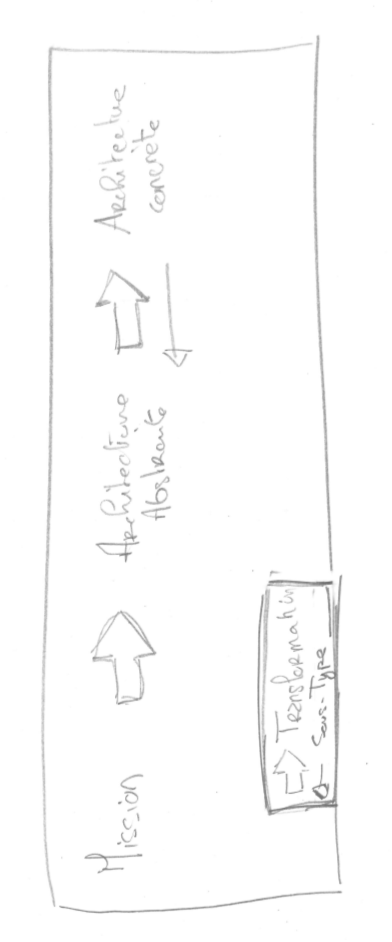
\includegraphics[scale=0.3, angle=-90]{construction-process}
  \begin{itemize}
  	\item Entender las ventajas y desventajas de distintos m�todos de optimizaci�n de la gradiente de descenso.
	\item Obtener la capacidad de discriminar entre distintos m�todos de optimizaci�n.
	\item Lograr un mejor entendimiento de las redes neuronales profundas.
  \end{itemize}
\end{frame}


\section{Marco Te�rico}
\subsection{Aprendizaje Autom�tico}
\begin{frame}{Aprendizaje Autom�tico}
	Se encarga consiste aprenden a identificar patrones en un conjunto de
	datos. A medida que se realiza este aprendizaje, la m�quina podr� ser capaz
	de realizar una predicci�n o tomar decisiones sin haber estado programada
	expl�citamente para realizar esta tarea.\\
	El Aprendizaje Autom�tico puede ser divido de la siguiente forma:
	\begin{itemize}
		\item Aprendizaje Supervisado
		\item Aprendizaje No Supervisado
		\item Aprendizaje por Refuerzo
	\end{itemize}
\end{frame}
\begin{frame}{Aprendizaje Supervisado}
	\begin{itemize}
		\item Regresi�n Lineal
		\item Regresi�n Log�stica 
		\item Clasificaci�n
	\end{itemize}
\end{frame}
\begin{frame}{Aprendizaje No Supervisado}
	\begin{itemize}
		\item 
	\end{itemize}
\end{frame}

\begin{frame}{Aprendizaje por Refuerzo}
\begin{figure}[H]
	\begin{center}
		\smartdiagramset{circular distance=2cm,
			font=\large,
			text width=1.6cm,
			module minimum width=1.8cm,
			module minimum height=0.5cm,
			arrow tip=to}
		\smartdiagram[circular diagram]{Agente,Accion, entorno,refuerzo}
		
	\end{center}
	\caption{Esquema de aprendizaje por refuerzo }
	\label{refuerzo}
\end{figure}
\end{frame}
\subsection{Redes Neuronales}
\begin{frame}{Redes Neuronales Artificiales}
Estas redes toman como inspiraci�n la arquitectura
del cerebro para la construcci�n de sistemas inteligente.
Actualmente son la base para el desarrollo de la inteligencia artificial.

\end{frame}
\begin{frame}{Comparaci�n neuronas biol�gicas y artificiales}
	\begin{figure}
		\centering
		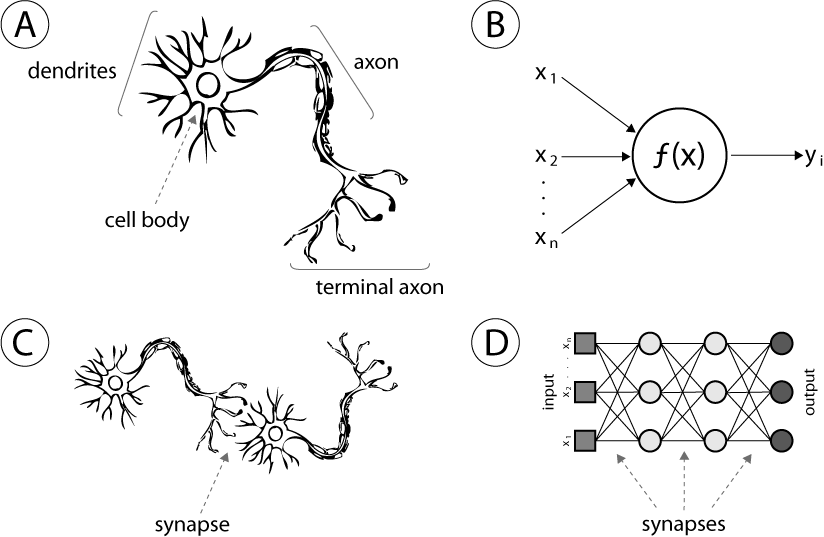
\includegraphics[width=0.6\textwidth]{figures/ANN.png}
		\caption{Redes neuronales biol�gicas y artificiales }
			\label{neuronas}
	\end{figure} 
\end{frame}

\begin{frame}{Redes neuronales Prealimentadas}
Es un tipo de red neuronal m�s simple que existe. Esta red puede clasificarse en:

\begin{itemize}
	\item Perceptron simple
	\item Perceptron Multicapas
	\item Redes neuronales convolucionales
\end{itemize}
\end{frame}
\begin{frame}{Esquema Redes neuronales Prealimentadas}
\begin{figure}[H]
	\centering
	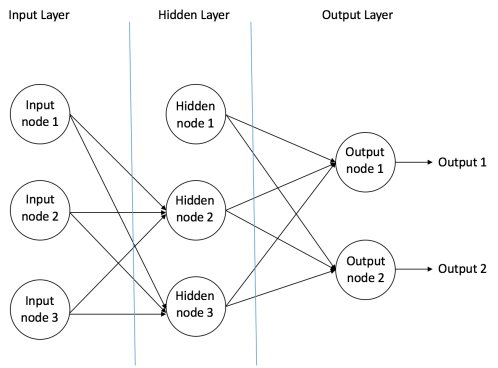
\includegraphics[width=0.7\textwidth]{figures/esquemaff.png}
	\caption{Esquema de Redes Neuronales Prealimentadas }
	\label{neuronasredes}
\end{figure} 
\end{frame}
\begin{frame}{Back Propagation}
	
\end{frame}
\begin{frame}{Redes Neuronales Convolucionales}

\end{frame}

\begin{frame}{Capas de una red neuronal convolucional}
	\begin{itemize}
		\item Input Layer
		\item Convolutional Layer
		\item Pooling Layer
		\item Fully Conected Layer
		\item Output Layer
	\end{itemize}
	
\end{frame}

\section{M�todos de Optimizaci�n}

\begin{frame}{Gradiente de Descenso}
	
\end{frame}

\begin{frame}{Variantes de la Gradiente de Descenso}
	Existen 3 variantes de la gradiente de descenso:
	\begin{itemize}
		\item Batch gradient descent
		\item Stochastic gradient descent
		\item Mini-batch gradient descent
	\end{itemize}

\end{frame}

\begin{frame}{M�todos para optimizar la gradiente de descenso}
	\begin{itemize}
		\item Momentum
		\item Nesterov Momentum 
		\item Adagrad
		\item RMSprop
		\item Adam
	\end{itemize}
\end{frame}
\subsection{Momentum}
\begin{frame}{Momentum}
	\begin{equation}
	\label{mbgds}
	\begin{aligned}
	\nu_{t}&=\gamma \nu_{t-1} +  \eta \nabla_{\theta} J(\theta)\\
	\theta &= \theta -\nu_{t}
	\end{aligned}
	\end{equation}
\end{frame}
\subsection{Nesterov}
\begin{frame}{Nesterov}
	\begin{equation}
	\label{mbgds}
	\begin{aligned}
	\nu_{t}&=\gamma \nu_{t-1} + \eta \nabla_{\theta} J(\theta- \gamma \nu_{t-1})\\
	\theta &= \theta -\nu_{t}
	\end{aligned}
	\end{equation}
\end{frame}
\subsection{Adagrad}
\begin{frame}{Adagrad}
	\begin{equation}
		\label{adagrad1}
		\begin{aligned}
		g_{t,i}&=\nabla_{\theta} J(\theta_{t,i})\\
		\theta_{t+1,i} &= \theta_{t,i} -\eta \cdot g_{t,i}
		\end{aligned}
	\end{equation}
	
	\begin{equation}
		\label{adagrad2}
		\begin{aligned}
		\theta_{t+1,i} &= \theta_{t,i} - \frac{\eta}{\sqrt{G_{t,ii}+\epsilon}} \cdot g_{t,i}
		\end{aligned}
	\end{equation}
\end{frame}
\subsection{RMSprop}
\begin{frame}{RMSprop}
	\begin{equation}
		\label{RMS}
		\begin{aligned}
		E[g^2]_{t} &= \gamma E[g^2]_{t-1} + (1-\gamma)g^{2}_{t}\\
		\theta_{t+1} &= \theta_{t} - \frac{\eta}{\sqrt{E[g^2]_{t} +\epsilon }} g_{t}
		\end{aligned}
	\end{equation}
\end{frame}
\subsection{Adam}
\begin{frame}{Adam}
	\begin{equation}
		\label{adam1}
		\begin{aligned}
		m_{t} &= \beta_{1} m_{t-1} +(1-\beta_{1})g_{t} \\
		v_{t} &= \beta_{2} v_{t-1} +(1-\beta_{2})g_{t}^2
		\end{aligned}
	\end{equation}
\end{frame}
\section{Resultados}
\begin{frame}{Resultados}
	Para obtener nuestros resultados utilizamos 2 datasets:
	\begin{itemize}
		 \item CIFAR 10
		 \item CIFAR 100
	\end{itemize}
	
\end{frame}
\begin{frame}{Resultados CIFAR-10}
	
\end{frame}

\begin{frame}{Resultados CIFAR-100}
	
\end{frame}
\section{Conclusiones y Trabajos Futuros}

\begin{frame}{Conclusiones}

\end{frame}

\begin{frame}{Trabajos Futuro}
	
\end{frame}

\end{document}